\documentclass[a4paper,12pt]{report}
\usepackage{graphicx}
\usepackage{titlesec}
\titleformat{\chapter}{}{}{0em}{\bf\LARGE}
\usepackage[utf8]{inputenc}
% Title Page
\title{Middle East Technical University\\Department of Physics\\PHYS222 Optics and Waves Laboratory\\\textbf{Experiment OW-3 Diffraction and Interference\\Laboratory Report}}

\author{Oğuzhan ÖZCAN\\1852334\\\\Partner: İnci SAİM\\\\Teaching Assistant: Kamil ÇINAR}


\begin{document}
\maketitle
\tableofcontents
\listoffigures
\listoftables
\chapter{Theory}
When an opaque object is placed between a point source of light and white screen, it is obvious that the shadow which is produced by object departs from the perfect sharpness as predicted by geometrical optics. If we look at this examination more closely shadow edges reveals that some light goes over into dark zone of the geometrical shadow. This phonemena known as \textit{diffraction}. The first detailed publishing about diffraction published by Francesco Grimaldi in the 1600s [1]. If there is an obstacle which is encounter by light, either transparent or opaque, a region of the wavefront is altered in amplitude or phase, diffraction will occur \footnote{Answer to Teaching Assistant's question.}.  For example, sound waves bend around corners much more than light does. That is  why we can hear but not see around corners. For a given type of waves, such as sound waves, how much the waves diffract depends on two factors: the size of the obstacle or opening in the obstacle and the wavelength. 
\begin{figure}[h!]
\centering
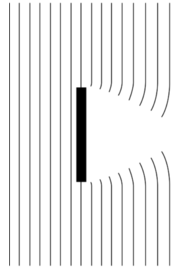
\includegraphics[width=0.3\linewidth, height=0.19\textheight]{obstacle}
\caption{Diffraction caused by an obstacle}
\label{fig:obstacle}
\end{figure}
At this point we have to clarify that diffraction is minor if the length of the obstacle or opening is greater than the wavelength and diffraction is major if the length of the obstacle or opening is less than the wavelength. The essential features of diffraction phenomena can be explained more widely by \textit{Huygens' principle}. This phenomena states that \textit{propagation of a light wave can be predicted by assuming that each point of the wave front acts as the source of a secondary wave that spreads out in all direction} [2]. 
\begin{figure}[h!]
\centering
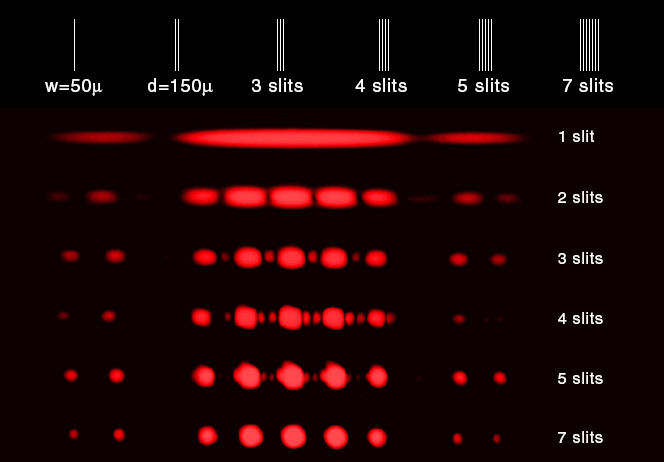
\includegraphics[width=0.8\linewidth, height=0.32\textheight]{diffraction}
\caption{An illustration for different numbers of slits}
\label{fig:diffraction}
\end{figure}
When we investigate diffraction more widely we should look at \textit{Fraunhofer} and \textit{Fresnel} diffraction. When the source source and observing plane are effectively at an infinite distance from the diffracting apertures, diffraction at finite distances is called \textit{Fresnel diffraction}. To understand the Huygens-Fresnel principle firstly we should give attention to the Fresnel Approximation. 
\begin{center}
	E (x,y,z)$\cong - \frac{ie^{ikz}e^{i\frac{k}{2z}(x^{2}+y^{2})}}{\lambda z}\int\int E(x',y',0)e^{i\frac{k}{2z}(x'^{2}+y'^{2})e^{-i\frac{k}{z}(xx'+yy')}}dx'dy'$ 
\end{center}
Previous equation known as Fresnel approximation. This approximation is valid when the observer is said to be in the region of Fresnel diffraction, or equivalently in the near field of the aperture [3].\\\\
Another important topic about diffraction is Fraunhofer diffraction. For a single slit incident plane waves are produced by placing
a monochromatic source at the focus of a positive lens. These waves are
incident normally on an opaque plane sheet pierced by a single long slit.
Beyond this sheet another positive lens images the diffraction pattern
onto a screen in its focal plane. The use of lenses brings the source and
image plane in from infinity, so making a compact experimental setup
with which to observe Fraunhofer diffraction. 
\begin{figure}[h!]
\centering
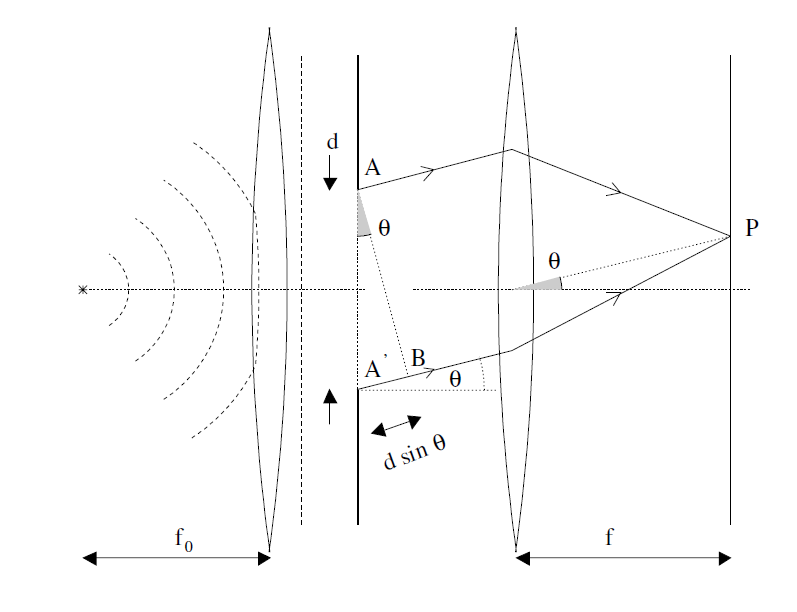
\includegraphics[width=0.9\linewidth, height=0.5\textheight]{fraunhofer}
\caption{Fraunhofer diffraction at a finite width slit}
\label{fig:fraunhofer}
\end{figure}
\\
The explanation of the single-slit pattern lies in the interference of the Huygens
secondary wavelets which can be thought of as sent out from every point on the wave front at the instant that it occupies the plane of the slit. In this sence we have a new term which is interference.\\\\
When two beams of light cross each other they do not interfere with each other. However, at the point where two beams of light crossing we are expecting that the resultant amplitude and intensity may be different from sum of two light beams. This modification of intensity obtained
by the superposition of two or more beams of light we call as \textit{interference} [4]. If the resultant intensity is zero or less than expecting resultant then we have \textit{destructive} interference.  Destructive interference occurs when $\delta=\pm\pi,\pm 3\pi, \pm 5\pi, ...,$ and it is defined as 
\begin{center}
	$I_{min}=I_{1}+I_{2}-2\sqrt{I_{1}I_{2}}$
\end{center}
On the other hand, if we have greater intensity than expecting resultant then we have \textit{constructive} interference. Constructive interference occurs when $\delta=0,\pm 2\pi, \pm 4\pi, ...,$ and it is defined as
\begin{center}
	$I_{max}=I_{1}+I_{2}+2\sqrt{I_{1}I_{2}}$
\end{center}
Note that when $I_{1}=I_{2}=I_{0}$, $I_{min}=0$ and $I_{max}=4I_{0}$. About the constructive and destructive interference, Richard Feynman wrote this definition in his lecture notes; \textit{"We call it interference whether it is positive or negative.
(Interference in ordinary language usually suggests opposition or hindrance, but
in physics we often do not use language the way it was originally designed!) If the
interference term is positive, we call that case constructive interference, horrible
though it may sound to anybody other than a physicist! The opposite case is
called destructive interference"} [5]. 
\begin{figure}[h]
\centering
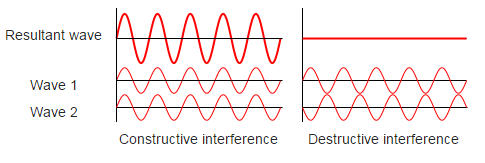
\includegraphics[width=0.8\linewidth, height=0.2\textheight]{interference}
\caption{Constructive and destructive interference of EM waves}
\label{fig:interference}
\end{figure}
The first experiments was done by Thomas Young. In the Young's experiment' setup (See Figure 1.5), a monochromatic light which has a wavelength $\lambda$, a tiny hole $S$ with a diameter $\delta$ of the order of fifty to hundred times the wavelength. 
\begin{figure}[h!]
\centering
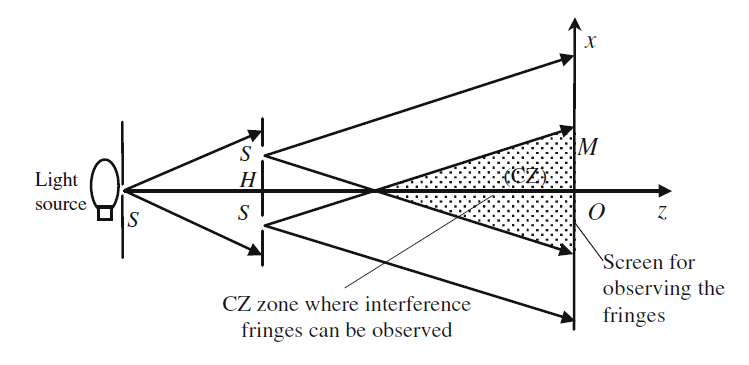
\includegraphics[width=0.9\linewidth, height=0.32\textheight]{young}
\caption{Young's experiment setup}
\label{fig:young}
\end{figure}
In this experiment Thomas Young define the following equations for interference fringes:
\begin{center}
Maxima: $\psi=\frac{2\pi}{\lambda}(MS_{2}-MS_{1})=(2p+1)\pi$ $\longrightarrow$ $(MS_{2}-MS_{1})=p\lambda$
\end{center}
\begin{center}
Minima: $\psi=\frac{2\pi}{\lambda}(MS_{2}-MS_{1})=(2p+1)\pi$ $\longrightarrow$ $(MS_{2}-MS_{1})=(2p+1)\lambda/2$
\end{center}
The above formulas define hyperboloids and each hyperboloids are labeled by the integer $p$ which called the \textit{order of interference} along the related hyperboloids [6].\\\\
Young's experiment is an example for Heisenberg uncertainity principle. Heisenberg uncertainity principle states that \textit{it is impossible to determine simultaneously
with unlimited precision the position and momentum of a particle} [7].
\begin{center}
	$\Delta p_{x} \Delta x=\frac{\hbar}{2}$
\end{center}
In Young’s double slit
experiment one may either know which slit the photon passes through
or one may observe the two slit interference pattern, but not both. If
the paths are indistinguishable then interference is seen, but if the path
is known interference no longer occurs. To be more precise we should look at wave-particle duality. The connection between the particle and wave properties of light is statistical. The probability of finding a photon in a given volume is simply related with instantaneous energy density of the electromagnetic wave
\begin{center}
	$PdV=IdV/\int IdV$
\end{center}
where \textit{P} is called the \textit{probability density} [8]. Young's double slit experiment provides a simple example about this relation \footnote{Answer to Teaching Assistant's question.}. 
\begin{figure}[h!]
\centering
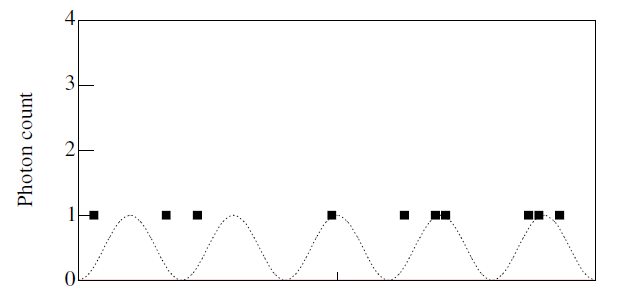
\includegraphics[width=0.9\linewidth, height=0.26\textheight]{young2slit}
\caption{Distrubution of photons in Young's two slit experiment for 10 photons}
\label{fig:young2slit}
\end{figure}



























\chapter{Data and Results}
\section{Part A: Single Slit}
\begin{table}[h]
	\begin{center}
\begin{tabular}{|c|c|c|}
	\hline Pattern & A & B \\ 
	\hline Width of the slit, a & 0.08 mm & 0.16 mm \\ 
	\hline Distance from the slit to the screen, L & 1.0 m & 1.0 m \\ 
	\hline Average distance between minima, $\bar{y}$ & 0.79 cm & 0.44 cm \\ 
	\hline $\bar{\lambda}=\frac{a\bar{y}}{L}$ & 635.0 nm & 710.0 nm \\ 
	\hline Error $\Delta y$ on $\bar{y}$ & 0.121 cm & 0.084 cm \\ 
	\hline Error $\Delta \bar{\lambda}$ on $\bar{\lambda}$ & 84.2 nm & 59.2 nm \\ 
	\hline $\lambda=\bar{\lambda}$$\pm$$\Delta\lambda$ & 550.8-719.2 nm & 650.8-769.2 nm \\ 
	\hline 
	\end{tabular} 
 
\end{center}
\caption{Sample Data for Single Slit Pattern}
\end{table}

\section{Part B: Double Slit}
\begin{table}[h]
	\begin{center}
		\begin{tabular}{|c|c|c|}
			\hline Pattern & C & D \\ 
			\hline Width of the slit, a & 0.04 mm & 0.08 mm \\
			\hline Distance between the center of the slits, d & 0.5 mm & 0.5 mm \\ 
			\hline Distance from the slit to the screen, L & 1.0 m & 1.0 m \\ 
			\hline Average distance between minima, $\bar{y}$ & 0.32 cm & 0.16 cm \\ 
			\hline $\bar{\lambda}=\frac{a\bar{y}}{L}$ & 475.5 nm & 790.0 nm \\ 
			\hline Error $\Delta y$ on $\bar{y}$ & 0.058 cm & 0.034 cm \\ 
			\hline Error $\Delta \bar{\lambda}$ on $\bar{\lambda}$ & 68.1 nm & 159 nm \\ 
			\hline $\lambda=\bar{\lambda}$$\pm$$\Delta\lambda$ & 407.4-543.6 nm & 631.0-949.0 nm \\ 
			\hline 
		\end{tabular} 
		
	\end{center}
	\caption{Sample Data for Double Slit Pattern}
\end{table}
In this experiment we have used a diode laser which produces a monochromatic beam with a wavelength of 650 nm. When we look our wavelength data we have a range from 407.4 nm and 949.0 nm. Our approximate value for wavelength almost same with theoretical one. That is why we can say that our data are valid. We can see this result by observing following graphs.
\begin{figure}[h]
\centering
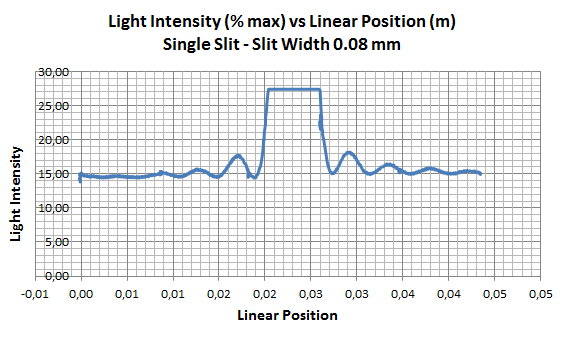
\includegraphics[width=1.0\linewidth, height=0.39\textheight]{1}
\caption{Light Intensity vs Linear Position for Single Slit (a=0.08mm)}
\label{fig:1}
\end{figure}
\begin{figure}[h]
\centering
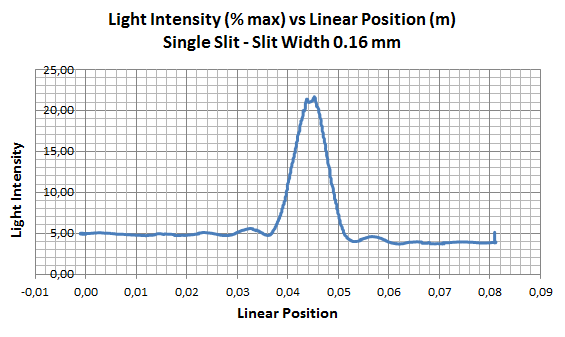
\includegraphics[width=1.0\linewidth, height=0.39\textheight]{2}
\caption{Light Intensity vs Linear Position for Single Slit (a=0.16mm)}
\label{fig:2}
\end{figure}
\begin{figure}[h]
\centering
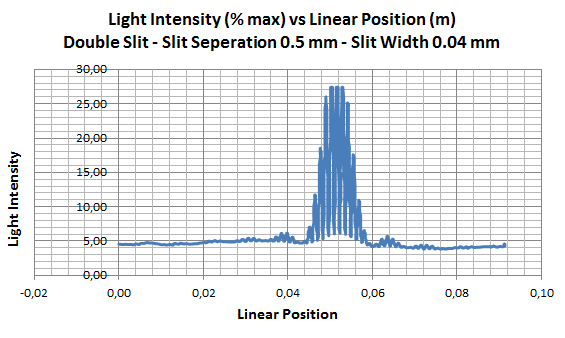
\includegraphics[width=1.0\linewidth, height=0.39\textheight]{3}
\caption{Light Intensity vs Linear Position for Double Slit (a=0.04mm)}
\label{fig:3}
\end{figure}
\begin{figure}[h]
\centering
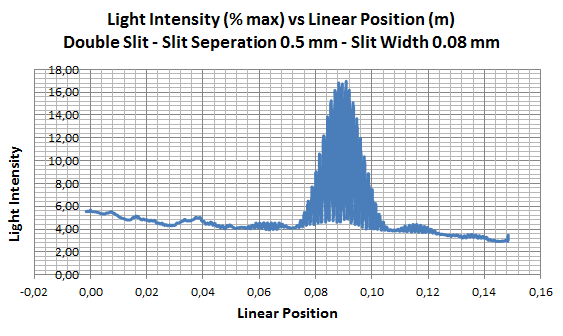
\includegraphics[width=1.0\linewidth, height=0.39\textheight]{4}
\caption{Light Intensity vs Linear Position for Double Slit (a=0.08mm)}
\label{fig:4}
\end{figure}



















\chapter{Discussion and Conclusion}
\textbf{1.What are the possible errors in the experiment?}\\
The most possible error cause may occur while moving light sensor. While moving light sensor we had some acceleration and deceleration and this caused some error. We can see this error in experiment graphs. Device which we took data has some error. Since we have some indoor light, this caused error also.\\\\
\textbf{2.What kind of approximation did you take into consideration while you were obtaining the physical quantities and how do they affect your results?}\\
We received experiment data via a computer based tool. That is why we do not have a lot of approximation. Only approximation is made while moving light sensor because we need to constant speed while reading intensity of light.\\\\ 
\textbf{3.What discrepancies did you encounter between the calculated quantities and theoretical or literature values?}\\
As mentioned in the lab manual we used a diode laser which has a wavelength of 650 nm. In single slit part we found that the wavelength as 635.0 nm. If we calculate percentage error
\begin{center}
	Percentage Error=$\frac{Theoretical Value-Experimental Value}{Theoretical Value}\times 100\%$
\end{center}
\begin{center}
	Percentage Error=$\frac{650.0-635.0}{650.0}\times 100\%=2.3\%$ nm
\end{center}
2.3 nm is a very small error when we compare theoretical value. That is why we can say that we do not have a certain discrepancy.\\\\ 
\textbf{4.What is your overall conclusion?}\\
To sum up, we studied interference and diffraction and their differences. We examine different results in single slit and double slit. In my opinion experiment is accomplished. We can see that our results have small amount of error. 
\chapter{Application}
\textbf{Blu-ray Disc}\\\\
Blu-ray Disc (BD) is a next-generation optical disc format supported by a group of the
world's leading consumer electronics and personal computer manufacturers, as well as
major studios. It was developed to enable high-definition (HD) video and new forms of
interactive entertainment. BD uses a shorter-wavelength blueviolet
laser that can focus to a much
smaller spot size compared to DVD’s
red laser. This allows data to be
packed more tightly and stored in
less space, giving a BD disc more
than five times the capacity of a DVD
Video disc.
While a DVD uses a 650 nm red laser, Blu-ray Disc uses a 405 nm "blue" laser diode. Note that even though the laser is called "blue", its color is actually in the violet range. The shorter wavelength can be focused to a smaller area, thus enabling it to read information recorded in pits that are less than half the size of those on a DVD, and can consequently be spaced more closely, resulting in a shorter track pitch, enabling a Blu-ray Disc to hold about five times the amount of information that can be stored on a DVD. The lasers are GaN (gallium nitride) laser diodes that produce 405 nm light directly, that is, without frequency doubling or other nonlinear optical mechanisms. Conventional DVDs use 650 nm red lasers, and CDs use 780 nm near-infrared lasers [9] [10].
\begin{figure}[h!]
\centering
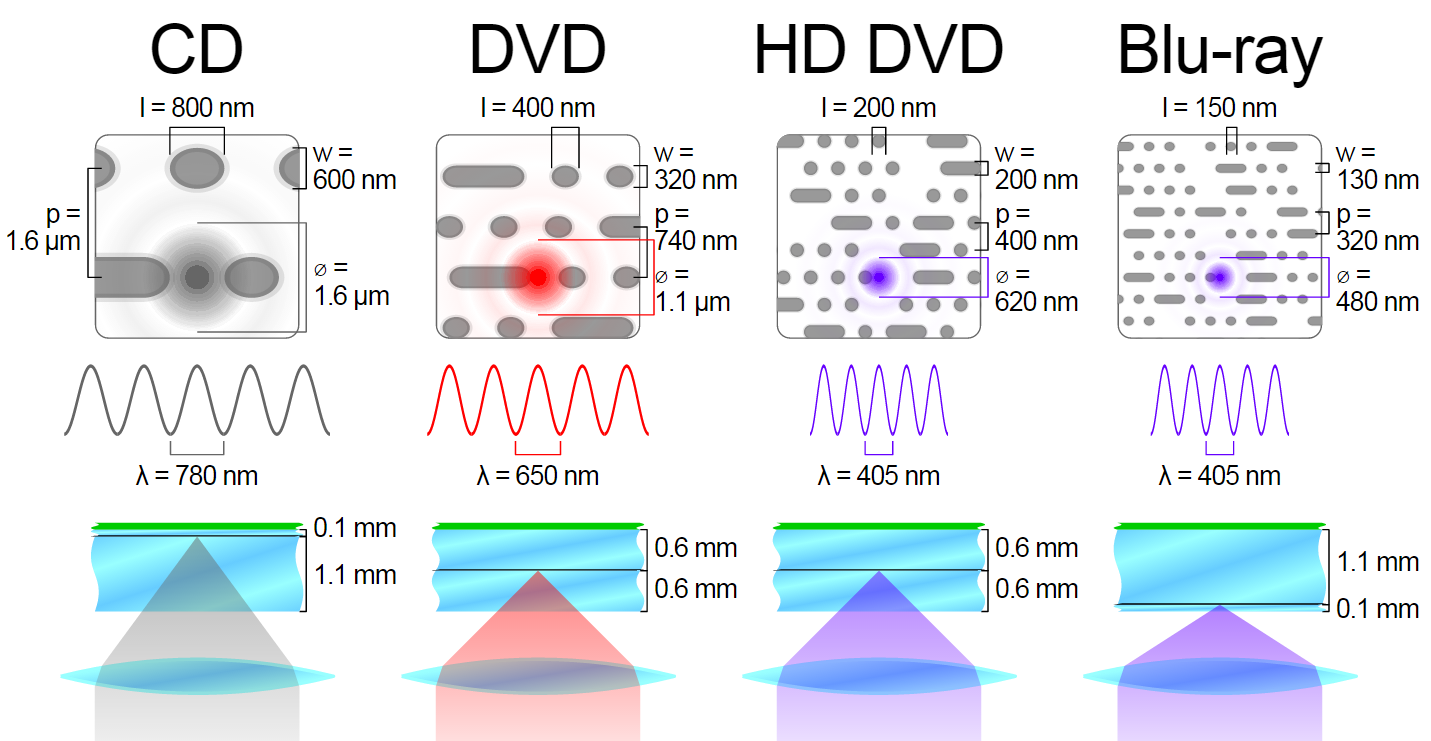
\includegraphics[width=0.6\linewidth, height=0.15\textheight]{blurat}
\caption{Comparison of CD, DVD, HD DVD and Blu-ray}
\label{fig:blurat}
\end{figure}

\chapter{References}
$[1]$ Hecht, E. (2002). \textit{Optics} (4th ed., p. 443). Reading, Mass.: Addison-Wesley.\\
$[2]$ Fowles, G. (1989). \textit{Introduction to Modern Optics} (2nd ed., Dover ed., p. 106). New York: Dover Publications.\\
$[3]$ Goodman, J. (1996). \textit{Introduction to Fourier Optics} (2nd ed., p. 69). New York: McGraw-Hill.\\
$[4]$ Jenkins, F., \& White, H. (2001). \textit{Fundamentals of Optics} (4th ed., p. 259). New York: McGraw-Hill.\\
$[5]$ Feynman, R., \& Leighton, R. (2011). \textit{The Feynman Lectures on Physics} (New millennium ed., p. 29-14). New York: Basic Books.\\
$[6]$  Chartier, G. (2005). \textit{Introduction to Optics} (p. 260). New York: Springer.\\
$[7]$ Serway, R., \& Moses, C. (2005). Modern physics (3rd ed., p. 174). Belmont, CA: Thomson Brooks/Cole.\\
$[8]$ Kenyon, I. (2008). \textit{The Light Fantastic: A Modern Introduction to Classical and Quantum Optics} (p. 342). Oxford England: Oxford University Press.\\
$[9]$ Blu-ray Disc: A New Dimension in High Definition. (n.d.). Retrieved April 26, 2015, from $http://www.pioneerelectronics.com/pio/pe/images/p\\ortal/cit-3424/292389922CES06-Blu-ray-brochure.pdf$\\
$[10]$ Blu-ray Disc (n.d.). Retrieved April 26, 2015, from $http://en.wikipedia\\.org/wiki/Blu-ray-Disc$






















































































\end{document}          
